% Options here are passed to the article class.
% Most common options: 10pt, 11pt, 12pt
\documentclass[10pt]{datasheet}

% Input encoding and typographical rules for English language
\usepackage[utf8]{inputenc}
\usepackage[english]{babel}
\usepackage[english]{isodate}

% tikz is used to draw images in this example, but you can
% also use \includegraphics{}.
\usepackage{graphicx}
\usepackage{float}
\usepackage{subcaption}

% These define global texts that are used in headers and titles.
\title{SG02: Global Clock Shulker Box Splitter}
\author{Obi}
\tags{splitting}
\date{21 December 2022}
\revision{Revision 3}
\begin{document}
\maketitle

\section{Features}

\begin{itemize}
\item{2wABt, fully hopper locked}
\item{Globally clocked, allowing the array to be paused in operation}
\item{Status outputs for activity, inactivity, \& empty box supply}
\end{itemize}

\section{Applications}

\begin{itemize}
\item{Dynamic sorting systems.}
\end{itemize}

\section{General Description}
Splits mixed boxes into smaller boxes of the same type. This design uses the hopper dueling mechanism for a "filter itemless" setup. It uses a global clock to allow for it to be paused during operation. Control wiring is comparatively tricky to do because of the global clock. Can lose empty boxes (although will not break) if they are input with no items. So don't do that. 

\vfill\break

\begin{figure}[H]
    \centering
    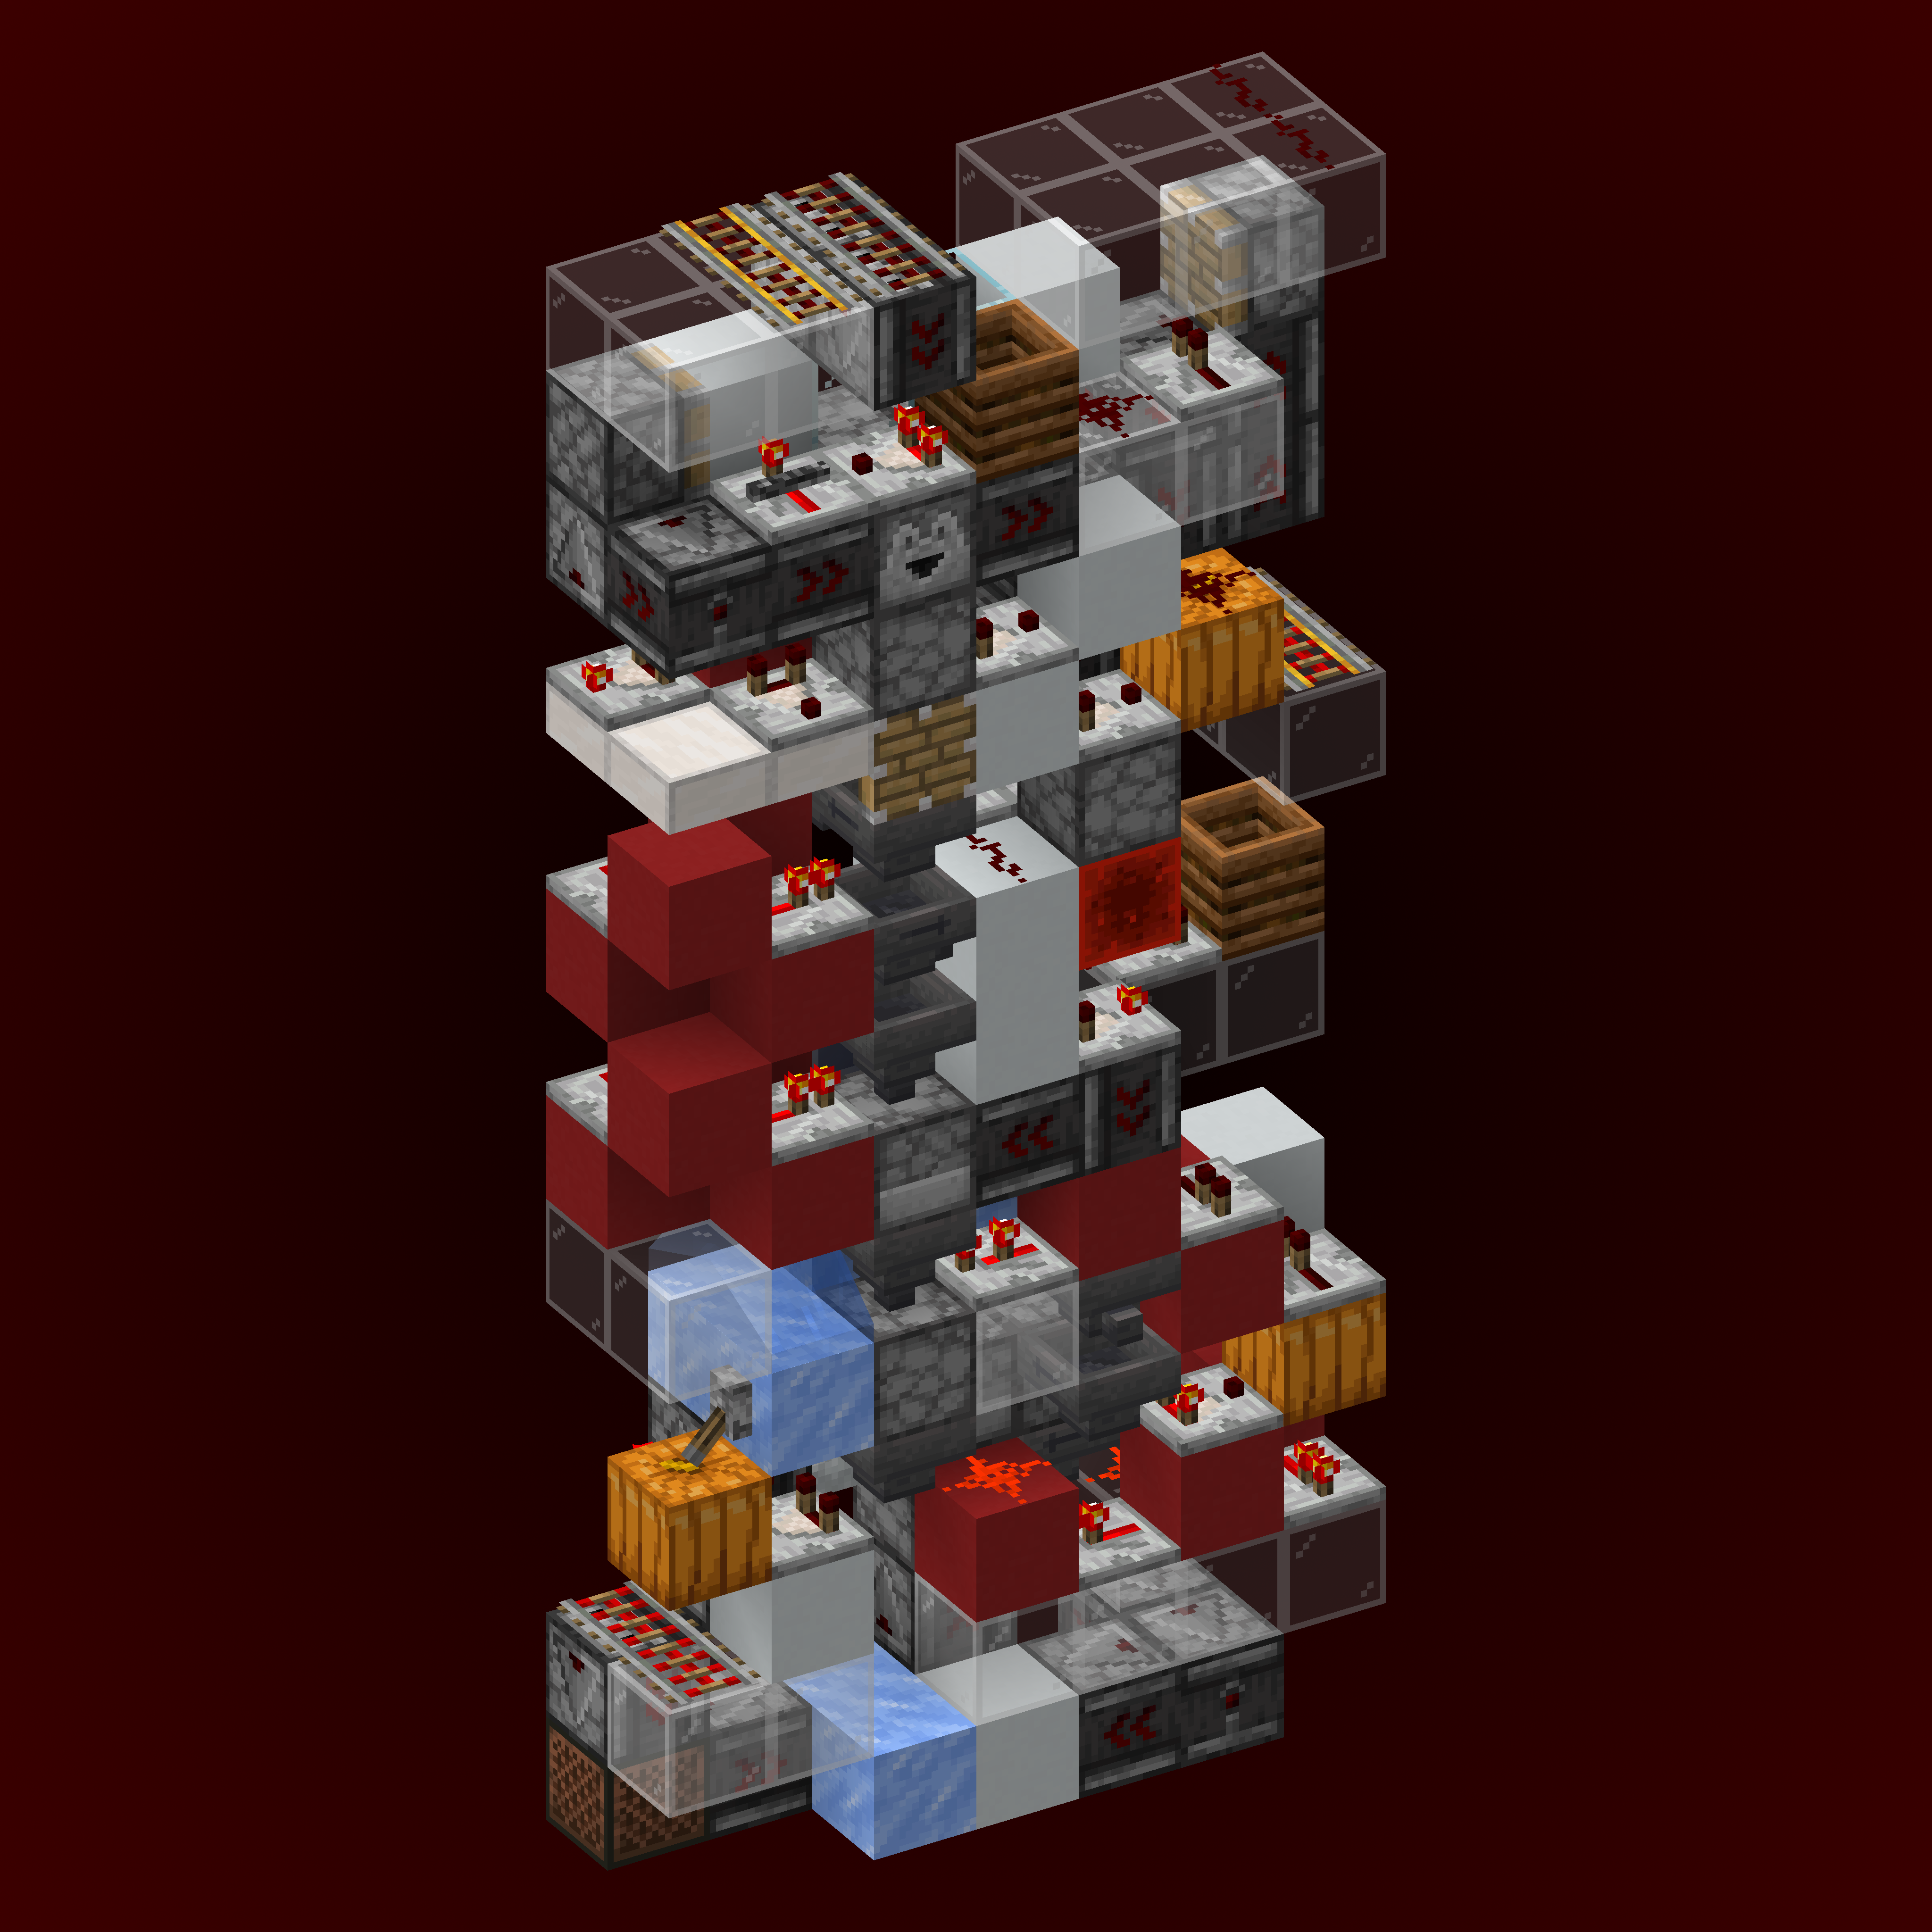
\includegraphics[width=0.48\textwidth]{globalclocksplitter1.png}
    \caption{\centering Shulker Box Splitter}
\end{figure}

% For wide tables, a single column layout is better. It can be switched
% page-by-page.
\onecolumn

\section{Device Specifications}

\begin{table}[H]
    \caption{Inputs}
    \begin{tabularx}{\textwidth}{l | c | X}
        \thickhline
        \textbf{Name} & \textbf{Range} & \textbf{Description} \\
        \hline
        Mixed boxes input & Box & Boxes to split. Boxes can contain any items. \\
        \thickhline
\end{tabularx}
\end{table}

\begin{table}[H]
    \caption{Outputs}
    \begin{tabularx}{\textwidth}{l | c | X}
        \thickhline
        \textbf{Name} & \textbf{Range} & \textbf{Description} \\
        \hline
        Split boxes output & Box & Boxes with same item types only \\
        \hline
        Unstackables output & Item & Unstackable items \\
        \thickhline
\end{tabularx}
\end{table}

\begin{table}[H]
    \caption{Device Specifications}
    \begin{tabularx}{\textwidth}{l | c c c | c | X}
        \thickhline
        \textbf{Parameter} & \textbf{Min.} & \textbf{Typ.} & \textbf{Max.} &
        \textbf{Unit} & \textbf{Conditions} \\
        \hline
        MC Version & 1.11 & - & - & MCV & Latest version at time of writing: 1.19.3\\
        \hline
        Dimensions & & 11 x 18 x 16 & & Blocks & \\
        \thickhline
\end{tabularx}
\end{table}

\section{Testing Data}
\begin{table}[H]
    \caption{Executed Tests}
    \begin{tabularx}{\textwidth}{l | X}
        \thickhline
        \textbf{Test} & \textbf{Result} \\
        \hline
        Splitting test & Device was able to split mixed boxes correctly. \\
        \thickhline
\end{tabularx}
\end{table}

\section{Download Information}
\begin{table}[H]
    \caption{Download Information}
    \begin{tabularx}{\textwidth}{l | l | l | X}
        \thickhline
        \textbf{Identifier} & \textbf{MC} & \textbf{File} & \textbf{Description} \\
        \hline
        SG02 & 1.17.1 & \href{https://github.com/Soontech-Annals/Archive/blob/8413f90a054b6c415703bae02badeba7541344f6/Archive/splitting/SG02\%20Global\%20Clock\%20Shulker\%20Box\%20Splitter/SG02\_Global\_Clock\_Shulker\_Box\_Splitter.litematic?raw=1}{SG02\_Global\_Clock\_Shulker\_Box\_Splitter.litematic} & Schematic of device. \\
        \hline
        \thickhline
    \end{tabularx}
\end{table}

\end{document}

